\documentclass{beamer}
\mode<presentation>
\usetheme{CambridgeUS}
\usepackage[russian]{babel}
\usepackage[utf8]{inputenc}
\usepackage[T2A]{fontenc}
\usepackage{sansmathaccent}

\usepackage{verbatim}
\usepackage{alltt}
\usepackage{graphicx}
\usepackage{minted}

\pdfmapfile{+sansmathaccent.map}
\title[Язык C]{Сокеты}
\author{Наумов Д.А., доц. каф. КТ}
\date[10.09.2019] {Операционные системы и системное программное обеспечение, 2020}

\begin{document}

%ТИТУЛЬНЫЙ СЛАЙД
\begin{frame}
  \titlepage
\end{frame}
  
%СОДЕРЖАНИЕ ЛЕКЦИИ
\begin{frame}
  \frametitle{Содержание лекции}
  \tableofcontents  
\end{frame}

\section{Введение}

\begin{frame}
	\begin{block}{Сокеты}
		это механизм межпроцессного взаимодействия, который позволяет обмениваться данными между приложениями, выполняемыми как локально, так и на разных компьютерах, соединенных по сети.
	\end{block}         
	\begin{itemize}
		\item сокеты фигурируют в виде \textit{файловых дескрипторов}, над которыми можно осуществлять обычные операции чтения-записи;
		\item набор действий, подготавливающих файловый дескриптор к использованию, несколько сложнее, чем в случае с обычными файлами;
		\item при взаимодействии посредством сокетов процессы рассматриваются по схеме \textit{<<клиент — сервер>>};
		\item процесс-сервер устанавливает <<правила общения>> и предлагает всем желающим межпроцессное взаимодействие.
\end{itemize}

    Сокет создается с применением системного вызова \texttt{socket()}; вся дальнейшая работа с сокетом выполняется с помощью дескриптора, возвращенного этим вызовом:
    
    \texttt{fd = socket(domain, type, protocol);}
\end{frame}

\begin{frame}
	\begin{figure}[h]
		\centering
		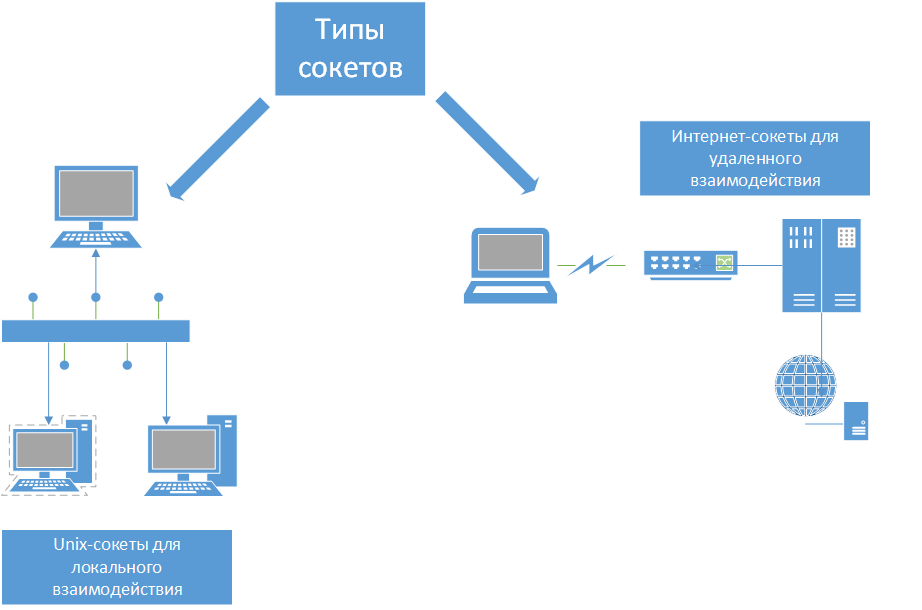
\includegraphics[scale=0.5]{images/lec12-pic01.png}
	\end{figure}
\end{frame}

\begin{frame}{Домены сокетов}
    Сокеты существуют внутри домена взаимодействия, определяющего:
    \begin{itemize}
        \item способ идентификации сокета (то есть формат его «адреса»);
        \item диапазон взаимодействия (то есть находятся ли приложения в одной системе или на разных компьютерах, соединенных по сети).
    \end{itemize}
    
    Современные операционные системы поддерживают как минимум домены следующих видов:
    \begin{itemize}
        \item UNIX-домен (AF\_UNIX) позволяет взаимодействовать приложениям, находящимся на одном компьютере;
        \item IPv4-домен (AF\_INET) позволяет взаимодействовать приложениям, которые выполняются на разных компьютерах, соединенных по сети на основе протокола IPv4;
        \item IPv6-домен (AF\_INET6) позволяет взаимодействовать приложениям, выполняемым на разных компьютерах, соединенных по сети на основе протокола IPv6.
    \end{itemize}
\end{frame}

\begin{frame}{Домены сокетов}
    \begin{figure}
    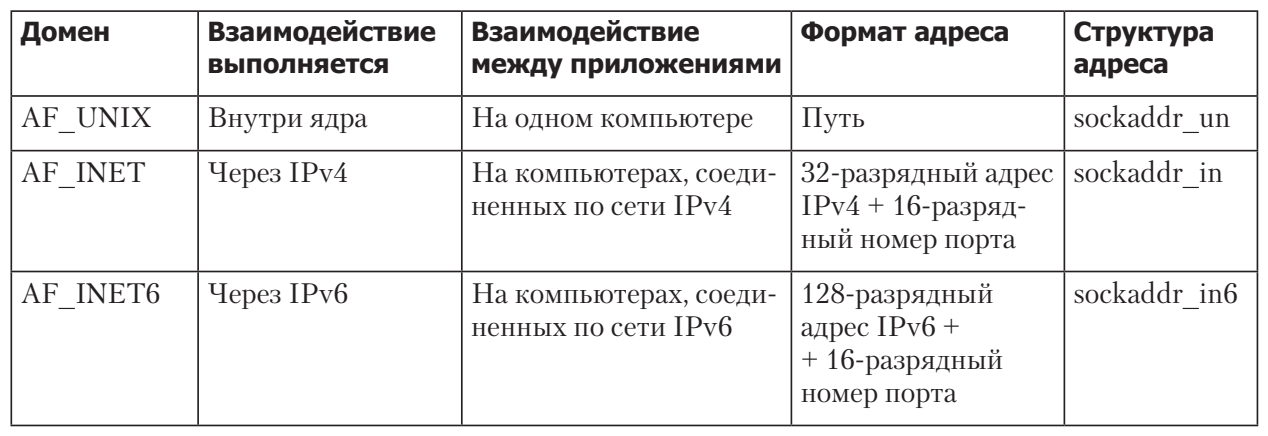
\includegraphics[scale=0.35]{images/domains.png}
    \end{figure}
\end{frame}

\begin{frame}
    Любая реализация предоставляет как минимум два вида сокетов:
	\begin{figure}[h]
		\centering
		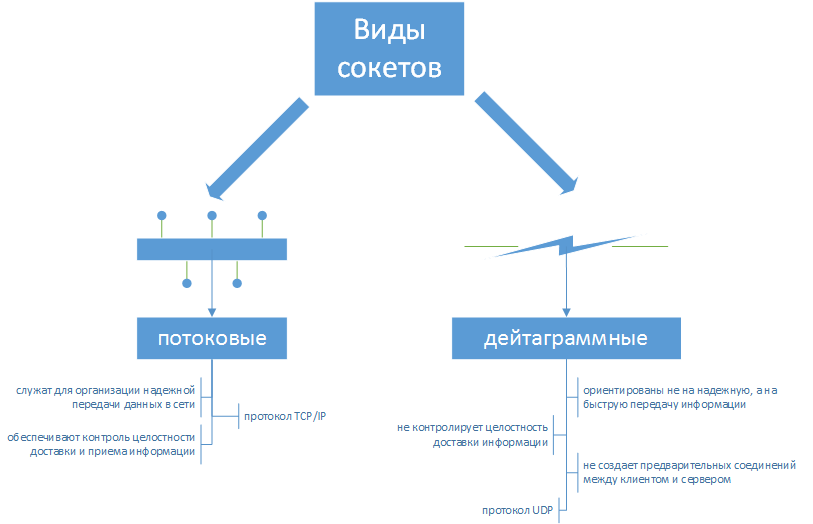
\includegraphics[scale=0.5]{images/lec12-pic04.png}
	\end{figure}
	Эти две разновидности поддерживаются как в UNIX-, так и в интернет-доменах.
\end{frame}

\begin{frame}{Потоковые сокеты}
    Потоковые сокеты (SOCK\_STREAM) предоставляют надежный, двунаправленный канал взаимодействия на основе байтового потока.
    \begin{itemize}
        \item \textit{надежный} -- мы гарантируем одно из двух: либо передаваемые данные будут доставлены невредимыми приложению-адресату, либо мы получим уведомление о возможном сбое при передаче;
        \item \textit{двунаправленный} -— данные могут передаваться между сокетами в любом направлении;
        \item \textit{байтовый поток} — сообщения не имеют границ.
    \end{itemize}
    
    Потоковые сокеты работают парами, соединяясь друг с другом, поэтому их называют ориентированными на соединение. 
    
    В интернет-доменах потоковые сокеты задействуют протокол \textbf{TCP} (\textit{Transmission Control Protocol} -— протокол управления передачей).
\end{frame}

\begin{frame}{Датаграммные сокеты}
    Датаграммные сокеты (SOCK\_DGRAM) позволяют обмениваться данными в виде сообщений, которые называются датаграммами. 
    \begin{itemize}
    	\item датаграммные сокеты сохраняют границы сообщений, но не обеспечивают надежную передачу данных. 
    	\item сообщения могут приходить не в том порядке, дублироваться или вовсе теряться. 
    	\item датаграммные сокеты являются общим случаем сетевого взаимодействия, не требующего соединения. В процессе работы им не нужно соединяться с другими сокетами (этим они отличаются от потоковых). Они могут быть соединены друг с другом, но по своей семантике данная процедура некоторым образом отличается от соединения потоковых сокетов.
    	\item в интернет-доменах датаграммные сокеты задействуют протокол UDP (User Datagram Protocol — протокол пользовательских датаграмм).   	
    \end{itemize}  
\end{frame}

\begin{frame}{TCP vs UDP}
    \begin{figure}
    
\includegraphics[scale=0.33]{images/tcp_udp.jpg}
    \end{figure}
\end{frame}

\section{Адреса сокетов: домен UNIX, интернет-сокеты}

\begin{frame}
  \frametitle{Содержание лекции}
  \tableofcontents[current]
\end{frame}

\begin{frame}[fragile]{Адреса сокетов}
    Адрес сокета в домене UNIX представляет собой путь к файлу, а структура, предназначенная для его хранения, имеет следующий вид:
    
\begin{minted}{c}
struct sockaddr_un {
    sa_family_t sun_family;  /* Всегда равно AF_UNIX */
    char sun_path[108];  /* Путь к сокету */
};
\end{minted}
    \begin{itemize}
    	\item Для привязки сокета UNIX-домена к адресу нужно инициализировать структуру \texttt{sockaddr\_un}, передать указатель на нее аргументу \texttt{addr} вызова \texttt{bind()} и указать \texttt{addrlen} в качестве размера этой структуры.
    	\item Привязывая сокет домена UNIX, вызов \texttt{bind()} создает запись в файловой системе.  Сам файл помечается как сокет.
    \end{itemize}    
\end{frame}

\begin{frame}{Привязка сокета домена UNIX}
    Необходимо отметить несколько моментов, касающихся привязки сокетов UNIX-домена.
    \begin{itemize}
        \item Сокет нельзя привязать к существующему пути.
        \item Обычно сокет привязывают к полному пути для фиксации его местоположения в файловой системе.
        \item Сокет можно привязать только к одному пути; и наоборот — путь может быть привязан только к одному сокету.
        \item Сокет нельзя открыть с помощью вызова \texttt{open()}.
        \item Когда сокет больше не нужен, его запись в файловой системе можно удалить, используя такие вызовы, как \texttt{unlink()} или \texttt{remove()}.
    \end{itemize}
\end{frame}

\begin{frame}[fragile]{Привязка сокета домена UNIX}
\begin{minted}{c}
const char *SOCKNAME = "/tmp/mysock";
struct sockaddr_un addr;
int sfd = socket(AF_UNIX, SOCK_STREAM, 0); /* Создаем сокет */
if (sfd == -1)
    return -1; /* Ошибка создания сокета */

/* Очищаем структуру */
memset(&addr, 0, sizeof(struct sockaddr_un));
addr.sun_family = AF_UNIX; /* Адрес домена UNIX */
strncpy(addr.sun_path, SOCKNAME, sizeof(addr.sun_path) - 1);
int s = bind(sfd, (struct sockaddr *) &addr, 
             sizeof(struct sockaddr_un));
if (s == -1)
    return -1; /* Ошибка привязки сокета */
\end{minted}
\end{frame}

\begin{frame}[fragile]{Привязывание адреса: локальное взаимодействие}
	При локальном взаимодействии на основе Unix-сокетов в качестве второго аргумента bind() используется указатель на структуру sockaddr\_un с полями: 
	\begin{itemize}
		\item sun\_family - семейство адресов (константа AF\_LOCAL или AF\_UNIX);
		\item sun\_path - обычная строка, содержащая путь к файлу сокета.
	\end{itemize}
	Пример: socket1.c
	
	Проверка:
	\begin{alltt}
		\$ gcc -o socket1 socket1.c
		\$ ./socket1 mysocket
		Press <Enter> to continue...
	\end{alltt}
	Теперь откроем другое терминальное окно и посмотрим на наш сокет:
	\begin{alltt}
		\$ ls -l mysocket
		srwxr-xr-x 1 nn nn 0 2019-12-11 10:18 mysocket
	\end{alltt}
\end{frame}

\begin{frame}[fragile]{Назначение адресов: интернет-сокеты}
	При локальном взаимодействии на основе Unix-сокетов в качестве второго аргумента bind() используется указатель на структуру sockaddr\_in с полями: 
	\begin{itemize}
		\item sun\_family - семейство адресов (константа AF\_INET);
		\item sin\_addr - адрес сокета;
		\item sin\_port - порт сокета.
	\end{itemize}
	Поле sin\_addr - это приведенный к целому числу IP-адрес серверного узла. Пример:
	\begin{itemize}
		\item IP-адрес: 192.168.0.1
		\item 192 = b11000000		
		\item 168 = b10101000		
		\item   0 = b00000000		
		\item   1 = b00000001						
		\item IP-адрес: b11000000101010000000000000000001 = 0xC0A80001
	\end{itemize}	
\end{frame}

\begin{frame}[fragile]{Преобразование имени в адрес}
Система доменных имен (DNS, Domain Name System) сопоставляет IP-адресам удобочитаемые имена (домены). Для преобразования IP-адреса или доменного имени в числовой адрес используется функция gethostbyname():
	\begin{alltt}
		struct hostent * gethostbyname (const char * NAME)
	\end{alltt}
	\begin{itemize}
		\item адрес узла обычно находится в элементе host->h\_addr\_list[0] структуры hostent;
		\item аргумент NAME - это доменное имя или IP-адрес.
	\end{itemize}
	\begin{alltt}
		host = gethostbyname (argv[1]);
		if (host == NULL) \{
		    fprintf (stderr, "Unknown server");
		    return 1;
		\}
	\end{alltt}	
\end{frame}

\begin{frame}[fragile]{Назначение адресов: порты}
	\begin{block}{Порт}
		число, идентифицирующее сеанс межпроцессного взаимодействия.
	\end{block}
	\begin{itemize}
		\item в поле sin\_port структуры sockaddr\_in содержится 16-разрядный номер порта.
		\item порядок записи байтов и битов на конкретном компьютере может отличаться от той, что принята в сети общего пользования. 
		\item для преобразования локального числа в 16-разрядный <<сетевой>> формат необходима функция htons().
	\end{itemize}
\end{frame}

\section{Системные вызовы для работы с сокетами}

\begin{frame}
  \frametitle{Содержание лекции}
  \tableofcontents[current]
\end{frame}

\begin{frame}{Системные вызовы}
    Ключевые системные вызовы для работы с сокетами:
    \begin{itemize}
        \item Системный вызов \texttt{socket()} создает новый сокет.
        \item Системный вызов \texttt{bind()} привязывает сокет к адресу. Обычно он используется сервером для привязки сокета к общеизвестному адресу, чтобы клиенты могли его найти.
        \item Системный вызов \texttt{listen()} позволяет потоковому сокету принимать входящие соединения от других сокетов.
        \item Системный вызов \texttt{accept()} принимает соединение от удаленного приложения в «слушающий» потоковый сокет и опционально возвращает адрес удаленного сокета.
        \item Системный вызов \texttt{connect()} устанавливает соединение с другим сокетом.
    \end{itemize}
    
    Ввод/вывод через сокеты может быть выполнен с помощью традиционных операций \texttt{read()} и \texttt{write()} или же специальных системных вызовов таких как \texttt{recv(), recvfrom(), send(), sendto()}.
\end{frame}

\begin{frame}[fragile]{Создание сокета}
    Системный вызов \texttt{socket()} создает новый сокет.    
\begin{minted}{c}
#include <sys/socket.h>

int socket(int domain, int type int protocol);
// Возвращает файловый дескриптор или -1, если произошла ошибка
\end{minted}
	
	\begin{itemize}
		\item Аргументы \texttt{domain} и \texttt{type} обозначают соответственно домен соединения сокета и его тип. 
		\item Параметр \texttt{protocol} задает конкретный протокол, который работает с сокетом. 
		\item Обычно существует только один протокол, задающий конкретный тип сокета в определенном семействе протоколов, в этом случае \texttt{protocol} может быть определено, как 0.  
	\end{itemize}  
\end{frame}

\begin{frame}[fragile]{Привязывание к адресу}
    Системный вызов \texttt{bind()} привязывает сокет к заданному адресу.
\begin{minted}{c}
#include <sys/socket.h>

int bind(int sockfd, const struct sockaddr *addr, 
         socklen_t addrlen);
// Возвращает 0 при успешном завершении или -1 при ошибке
\end{minted}

	\begin{itemize}
    	\item Аргумент \texttt{sockfd} представляет собой файловый дескриптор, полученный из предыдущего вызова \texttt{socket()}. 
    	\item Аргумент \texttt{addr} является указателем на структуру, описывающую адрес привязки сокета. 
    	\item Тип структуры, передаваемой в этом аргументе, зависит от домена сокета. 
    	\item Аргумент \texttt{addrlen} обозначает размер структуры с адресом; он имеет тип \texttt{socklen\_t}, должен быть целым числом.
	\end{itemize}    
\end{frame}

\section{Потоковые сокеты}

\begin{frame}
  \frametitle{Содержание лекции}
  \tableofcontents[current]
\end{frame}

\begin{frame}[shrink]{Принцип работы}
    Принцип работы потоковых сокетов:
    \begin{enumerate}
        \item Системным вызовом \texttt{socket()} создается сокет. Чтобы приложения могли взаимодействовать друг с другом, каждое из них должно создать свой сокет.
        \item Прежде чем начать общение, приложения должны соединить свои сокеты. Это делается следующим образом.
        \begin{itemize}
            \item Одно приложение делает вызов \texttt{bind()}, чтобы привязать свой сокет к общеизвестному адресу, и затем вызывает \texttt{listen()} для уведомления ядра о своей готовности принимать входящие соединения.
            \item Другое приложение устанавливает соединение с помощью вызова \texttt{connect()}, указывая адрес сокета, к которому оно хочет подключиться. 
            \item Затем приложение, вызвавшее \texttt{listen()}, принимает соединение, используя вызов \texttt{accept()}. Вызов \texttt{accept()} блокируется, если сделать его до того, как другое приложение выполнит \texttt{connect()}.
        \end{itemize}
        \item Подключившись, можно передавать данные в обоих направлениях, пока одно из приложений не закроет соединение с помощью вызова \texttt{close()}. 
    \end{enumerate}
\end{frame}

\begin{frame}
	\begin{figure}[h]
		\centering
	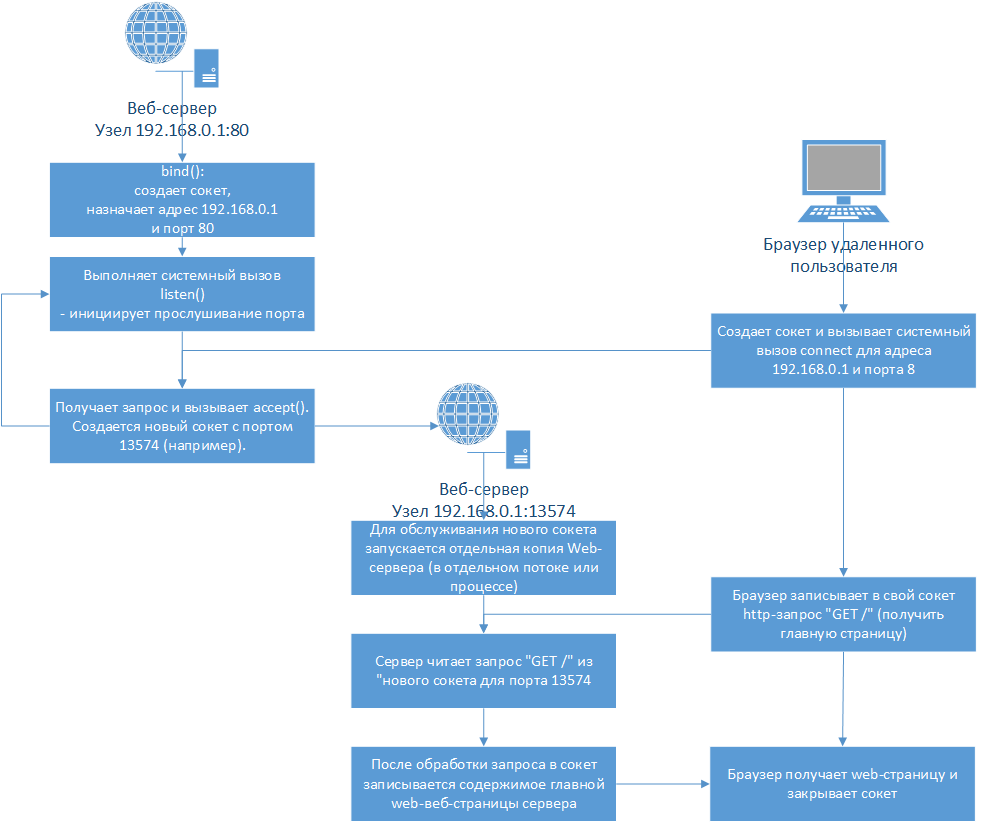
\includegraphics[scale=0.4]{images/lec12-pic05.png}
	\end{figure}
\end{frame}

\begin{frame}[fragile]{Соединение сокетов}
	При использовании потоковых сокетов между взаимодействующими процессами должно сначала установиться соединение.
	Для этого клиент вызывает системный вызов connect():
	\begin{minted}{c}
int connect (int sockfd, const struct sockaddr * addr,
             socklen_t addrlen);
	\end{minted}
	\begin{itemize}
		\item sockfd - это дескриптор сокета;
		\item addr - указатель на структуру, содержащую сведения об адресе сервера;
		\item addrlen - размер адресной структуры.		
	\end{itemize}
	Пример getwwwpage.c
	\begin{alltt}
		\$ gcc -o getwwwpage getwwwpage.c
		\$ ./getwwwpage rsreu.ru > index.html
	\end{alltt}	
\end{frame}

\begin{frame}[fragile]{Ожидание входящих соединений}
    Системный вызов \texttt{listen()} делает потоковый сокет \texttt{sockfd} пассивным. Впоследствии этот сокет будет использоваться для приема соединений от других (активных) сокетов.

\begin{minted}{c}
#include <sys/socket.h>
int listen(int sockfd, int backlog);
// Возвращает 0 при успешном завершении или -1 при ошибке
\end{minted}

	\begin{itemize}
		\item Вызов \texttt{listen()} нельзя применять к подключенным сокетам, для которых уже была успешно выполнена операция connect(), или к возвращенным вызовами \texttt{accept()}.
	\end{itemize}    			
\end{frame}

\begin{frame}[fragile]{Прослушивание сокета}
	Чтобы понять назначение аргумента \texttt{backlog}, следует отметить: 		
	\begin{itemize}
		\item Клиент может вызвать \texttt{connect()} до того, как сервер выполнит вызов \texttt{accept()}. 
		\item Данная ситуация приводит к возникновению отложенного соединения. Ядро должно записывать сведения о каждом отложенном запросе на подключение, чтобы впоследствии выполнить необходимые вызовы \texttt{accept()}. 
		\item Аргумент \texttt{backlog} позволяет ограничить количество таких отложенных соединений. 
	\end{itemize}    
	
	\begin{minted}{c}
if (listen (sock, backlog) == -1) {
    fprintf (stderr, "listen() error");
    return 0;
}
	\end{minted}
\end{frame}

\begin{frame}[fragile]{Прием соединения}
	\begin{itemize}
		\item Системный вызов listen() блокирует сервер до тех пор, пока какой-нибудь клиент не выдаст запрос на подключение. 
		\item Как только запрос поступил, сервер <<просыпается>>. 
		\item Если есть возможность обслужить запрос, то сервер вызывает системный вызов accept():
	\end{itemize}	
	
	Системный вызов \texttt{accept()} принимает входящее соединение на слушающем потоковом сокете \texttt{sockfd}.
\begin{minted}{c}
#include <sys/socket.h>
int accept(int sockfd, struct sockaddr *addr, 
           socklen_t *addrlen);
// Возвращает файловый дескриптор или -1, если произошла ошибка
\end{minted}

	\begin{itemize}
		\item sockfd - это дескриптор сокета;
		\item По адресу addr расположена структура, в которую помещаются адресные данные созданного соединения; 
		\item addrlen — адрес переменной, в которую помещается размер адресной структуры.
	\end{itemize}
\end{frame}

\begin{frame}[fragile]{Прием соединения}
	\begin{itemize}
		\item Вызов \texttt{accept()} создает новый сокет, который затем подключается к удаленному сокету, выполнившему вызов \texttt{connect()}. Слушающий сокет остается открытым и может использоваться для приема последующих соединений.
		\item Аргумент \texttt{addr} указывает на структуру, применяемую для возвращения адреса сокета.
		\item Аргумент \texttt{addrlen} указывает на целое число. Перед выполнением вызова оно должно быть инициализировано с помощью размера буфера, на который указывает \texttt{addr}. 
	\end{itemize}   
\end{frame}

\begin{frame}[fragile]
	Пример: socket2-server.c, socket2-client.c

	Вскоре после запуска сервер переходит в режим прослушивания сокета:
	\begin{alltt}
	\$ gcc -o socket2-server socket2-server.c
	\$ ./socket2-server
	\end{alltt}
	Откроем теперь другое терминальное окно и начнем передавать серверу запросы:
	\begin{alltt}
	\$ gcc -o socket2-client socket2-client.c
	\$ ./socket2-client Hello
	\$ ./socket2-client World
	\$ ./socket2-client Linux
	\end{alltt}	
	В исходном терминальном окне сервера будут выводиться соответствующие сообщения:
	\begin{alltt}
	>> Hello
	>> World
	>> Linux
	\end{alltt}	
	Сервер будет выводить сообщения, пока клиент не пошлет <<exit>>.
\end{frame}

\begin{frame}[fragile]{Соединение с удаленным сокетом}
    Системный вызов \texttt{connect()} соединяет активный сокет \texttt{sockfd}, со слушающим сокетом, чей адрес задан в виде аргументов \texttt{addr} и \texttt{addrlen}.
    
\begin{minted}{c}
#include <sys/socket.h>
int connect(int sockfd, const struct sockaddr *addr, 
            socklen_t addrlen);
// Возвращает 0 при успешном завершении или -1 при ошибке
\end{minted}
        	
    Если вызов \texttt{connect()} завершается неудачей и мы хотим повторить попытку соединения, то:
    \begin{itemize}
    	\item нужно закрыть имеющийся сокет, 
    	\item создать вместо него новый сокет 
    	\item с его помощью попытаться соединиться еще раз.
    \end{itemize}    
\end{frame}

\begin{frame}[fragile]{Закрытие соединения}
    Обычно для закрытия соединения на основе потоковых сокетов используется вызов close().

\begin{minted}{c}
#include <unistd.h>

int close(int fd);
// Возвращает 0 при успешном завершении или -1 при ошибке
\end{minted}
\end{frame}

\begin{frame}{Взаимодействие TCP-сокетов}
    \begin{figure}
    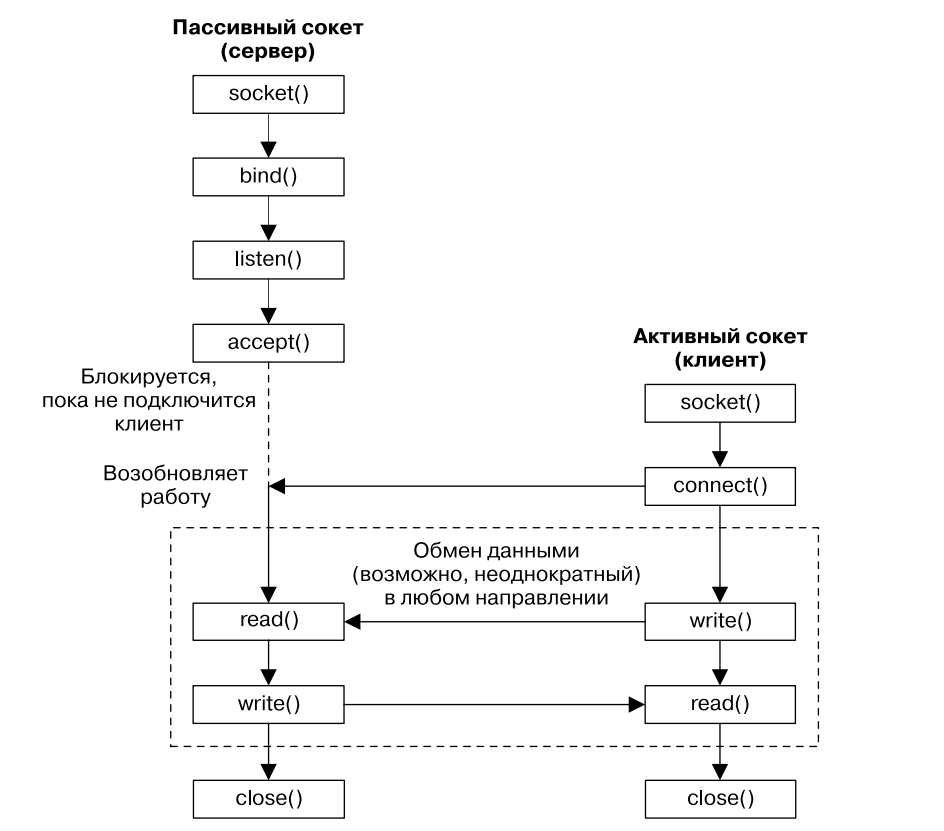
\includegraphics[scale=0.33]{images/tcp_communication.png}
    \end{figure}
\end{frame}

\section{Датаграммные сокеты}

\begin{frame}
  \frametitle{Содержание лекции}
  \tableofcontents[current]
\end{frame}

\begin{frame}[shrink]{Принцип работы}
    Принцип работы датаграммных сокетов:
    \begin{enumerate}
        \item Любое приложение, которое хочет отправлять или получать датаграммы, должно создать датаграммный сокет с помощью вызова \texttt{socket()}.
        
        \item Чтобы иметь возможность принимать датаграммы от других приложений, нужно привязать свой сокет к общеизвестному адресу, воспользовавшись вызовом \texttt{bind()}. Обычно это делает сервер, а клиент инициирует взаимодействие, отправляя по данному адресу свою датаграмму.
        
        \item Для отправки датаграммы приложение делает вызов \texttt{sendto()}. Он в качестве одного из своих аргументов принимает адрес удаленного сокета, которому предназначено сообщение.
        
        \item Чтобы получить датаграмму, приложение делает вызов \texttt{recvfrom()}, который может заблокироваться, если она еще не пришла. Данный вызов также позволяет определить адрес отправителя.
        
        \item Когда сокет больше не нужен, приложение закрывает его с помощью вызова \texttt{close()}.
    \end{enumerate}
\end{frame}

\begin{frame}[fragile]{Прием датаграмм}
    Системный вызов \texttt{recvfrom()} принимает датаграммы на датаграммный сокет.
    
\begin{minted}{c}
#include <sys/socket.h>
ssize_t recvfrom(int sockfd, void *buffer, size_t length,
                 int flags, struct sockaddr *src_addr, 
                 socklen_t *addrlen);
// Возвращает количество полученных байтов, 
// 0, если обнаружен конец файла, или -1 при ошибке
\end{minted}
	
	\begin{itemize}
	    \item Возвращаемое значение и первые три аргумента такие же, как у операции \texttt{read()}.
	    \item Четвертый аргумент, \texttt{flags}, представляет собой битовую маску, которая определяет специальные возможности ввода/вывода, связанные с сокетами.
	    \item Аргументы \texttt{src\_addr} и \texttt{addrlen} возвращают адрес удаленного сокета, с помощью которого была отправлена датаграмма. 
	\end{itemize}
\end{frame}

\begin{frame}[fragile]{Отправка датаграмм}
    Системный вызов \texttt{sendto()} отправляет датаграммы на датаграммный сокет.
    
\begin{minted}{c}
#include <sys/socket.h>
ssize_t sendto(int sockfd, const void *buffer, size_t length, 
              int flags, const struct sockaddr *dest_addr, 
              socklen_t addrlen);
// Возвращает количество отправленных байтов или -1 при ошибке
\end{minted}

	\begin{itemize}
	    \item Возвращаемое значение и первые три аргумента такие же, как у операции \texttt{write()}.
	    \item Четвертый аргумент, \texttt{flags}, представляет собой битовую маску, которая определяет специальные возможности ввода/вывода, связанные с сокетами.
	    \item Аргументы \texttt{dest\_addr} и \texttt{addrlen} описывают сокет, которому будет отправлена датаграмма.
	\end{itemize}
\end{frame}

\begin{frame}{Взаимодействие UDP-сокетов}
    \begin{figure}
    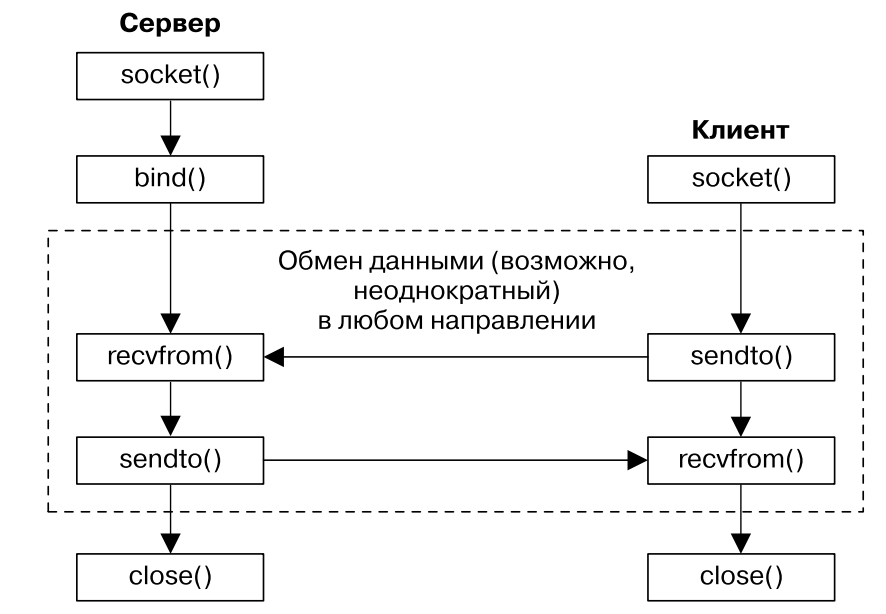
\includegraphics[scale=0.4]{images/udp_communication.png}
    \end{figure}
    Пример: \textit{socket3-server.c}, \textit{socket3-client.c}
\end{frame}

\begin{frame}{Вызов \texttt{connect()} для UDP-сокета}
    Датаграммные сокеты не нуждаются в соединении, однако при работе с ними тоже можно применять системный вызов \texttt{connect()}. Он заставляет ядро записать адрес удаленного сокета. Такие сокеты называются \textbf{соединенными}. 
    
    После соединения датаграммного сокета:
    \begin{itemize}
        \item датаграммы, отправляемые с помощью вызова \texttt{write()} (или \texttt{send()}), автоматически передаются заданному удаленному сокету;        
        \item мы можем читать только датаграммы, отправленные заданным удаленным сокетом.
    \end{itemize}
    
    Удаленный адрес соединенного датаграммного сокета можно изменить с помощью повторного вызова connect().
\end{frame}

\end{document}